\documentclass[border=3pt]{standalone}
% Preâmbulo compartilhado pelos diagramas TikZ da aula 4 de Navegação (Representação de Mapas)
\usepackage[T1]{fontenc}
\usepackage[utf8]{inputenc}
\usepackage{lmodern}
\usepackage{amsmath}
\usepackage{xcolor}
\usepackage{tikz}
\usetikzlibrary{arrows.meta,angles,quotes,decorations.pathmorphing,decorations.pathreplacing,calc,
                positioning,shapes.geometric,shapes.misc,backgrounds,fit,
                math}

% Paleta (mesma dos SVGs originais)
\definecolor{dblue}{HTML}{2A5B8C}
\definecolor{dorange}{HTML}{B3541E}
\definecolor{dgreen}{HTML}{4A7C59}
\definecolor{dred}{HTML}{9C4B4B}
\definecolor{dcream}{HTML}{F4F1EA}
\definecolor{dshade}{HTML}{DDD7C9}

% Função gaussiana (não normalizada por padrão de escala visual)
\pgfmathdeclarefunction{gauss}{3}{%
  \pgfmathparse{1/(#3*sqrt(2*pi))*exp(-((#1-#2)^2)/(2*#3^2))}%
}

% Estilos comuns (prefixo d... para não colidir com chaves internas do pgf)
\tikzset{
  >={Stealth[length=2mm]},
  dguide/.style={gray!55, dashed, line width=0.4pt},
  daxis/.style={gray!60, line width=0.7pt, ->},
  dbody/.style={fill=black!3, draw=black!80, line width=1pt},
  dacc/.style={draw=dblue, line width=1pt},
  dlbl/.style={black!55, font=\small},
  dsub/.style={black!45, font=\footnotesize},
  dstate/.style={circle, draw=black!80, fill=dcream, line width=1pt,
                 minimum size=17mm, font=\large, inner sep=1pt},
  dobs/.style={circle, draw=black!80, fill=dshade, line width=1pt,
               minimum size=14mm, font=\large, inner sep=1pt},
  dbox/.style={rounded corners=2pt, draw=black!80, fill=dcream, line width=1pt,
               align=center, inner sep=6pt},
  dop/.style={circle, draw=black!80, fill=white, line width=1pt,
              minimum size=6mm, inner sep=0pt, font=\small},
  dtrans/.style={->, dblue, line width=1pt},
  dmeas/.style={->, dorange, line width=1pt},
  dcurve/.style={line width=1pt, dblue},
  dcurveb/.style={line width=1.4pt, dorange},
}

\begin{document}
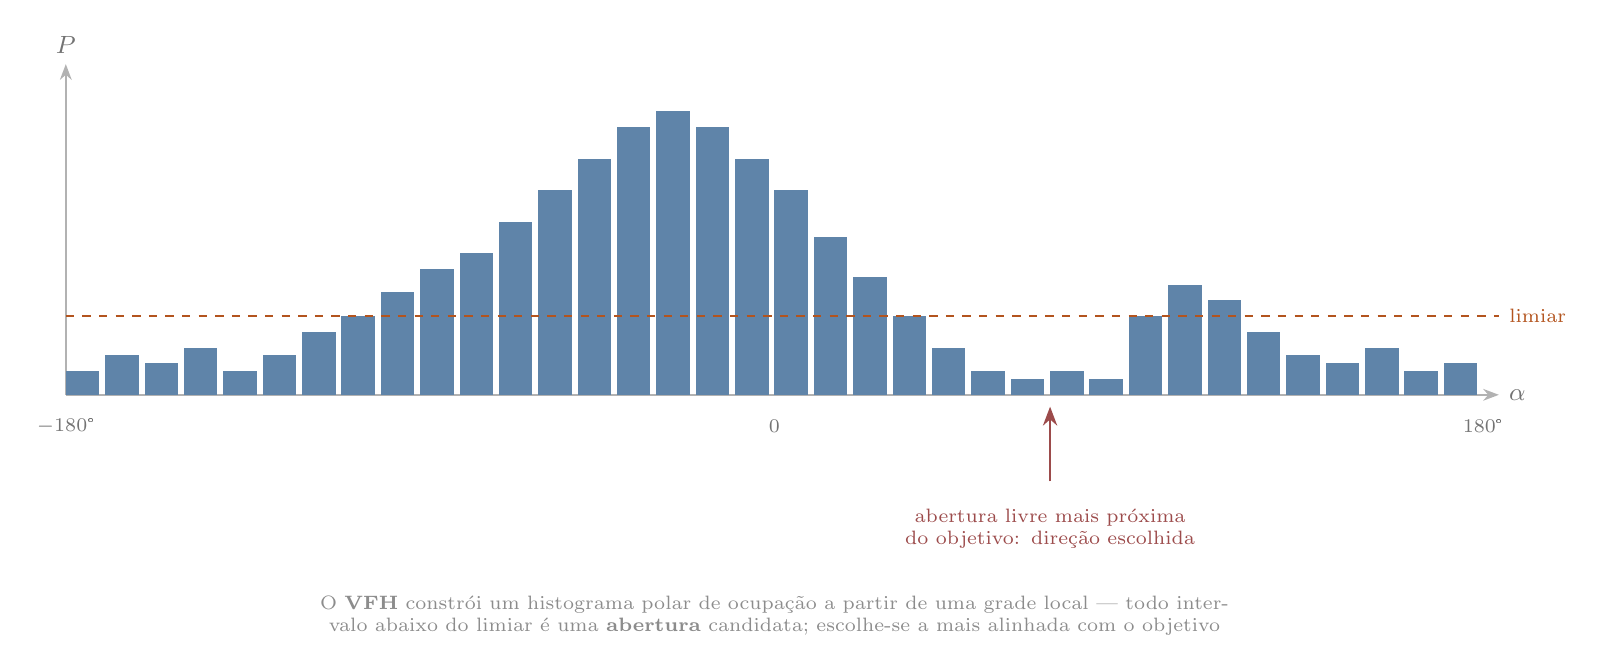
\begin{tikzpicture}[x=1cm,y=1cm]

  \def\bw{0.5}
  \def\heights{{
    0.3,0.5,0.4,0.6,0.3,0.5,
    0.8,1.0,1.3,1.6,1.8,
    2.2,2.6,3.0,3.4,3.6,3.4,3.0,
    2.6,2.0,1.5,1.0,0.6,
    0.3,0.2,0.3,0.2,
    1.0,1.4,1.2,0.8,
    0.5,0.4,0.6,0.3,0.4
  }}

  \draw[daxis] (0,0) -- (18.2,0) node[right, dlbl, font=\small] {$\alpha$};
  \draw[daxis] (0,0) -- (0,4.2) node[above, dlbl, font=\small] {$P$};

  \foreach \i in {0,...,35} {
    \pgfmathsetmacro{\h}{\heights[\i]}
    \fill[dblue!75] (\i*\bw,0) rectangle ++(\bw*0.85,\h);
  }

  \draw[dorange, dashed, line width=0.9pt] (0,1.0) -- (18.2,1.0)
    node[right, dorange, font=\scriptsize] {limiar};

  \node[dlbl, font=\scriptsize] at (0,-0.4) {$-180${\textdegree}};
  \node[dlbl, font=\scriptsize] at (9,-0.4) {$0$};
  \node[dlbl, font=\scriptsize] at (18,-0.4) {$180${\textdegree}};

  \draw[dred, line width=1pt, -{Stealth[length=2.4mm]}] (12.5,-1.1) -- (12.5,-0.15);
  \node[dred, font=\scriptsize, align=center, text width=4.2cm] at (12.5,-1.7) {abertura livre mais próxima do objetivo: direção escolhida};

  \node[dsub, font=\scriptsize, align=center, text width=17.5cm] at (9,-2.8)
     {O \textbf{VFH} constrói um histograma polar de ocupação a partir de uma grade local --- todo intervalo abaixo do limiar é uma \textbf{abertura} candidata; escolhe-se a mais alinhada com o objetivo};

\end{tikzpicture}
\end{document}
